\chapter{Integration with Process Simulate}
\label{ch:integration}
\graphicspath{{chapters/Integration/}}

What is process simulate, why we chose it, who uses it and why.

What it allows us to do

Introduce compound operations paths and points

\section{Writing Plug-ins}

how to write a plugin

Tools used and why

\section{Plug-in Architecture}

\section{Plug-in Features}
How to find it in UI

features available

\section{Plug-in Modules}

\section{Optimization Process}

The optimization process consists of the main optimization routine and several modules that provide the required functionality for the algorithm which then glues it together. This chapter will first explain the optimization process and then focus on the supporting modules in the sub-sections. \\

\begin{figure}[ht]
	\caption{Begin Optimization Dialog}
	\centering
	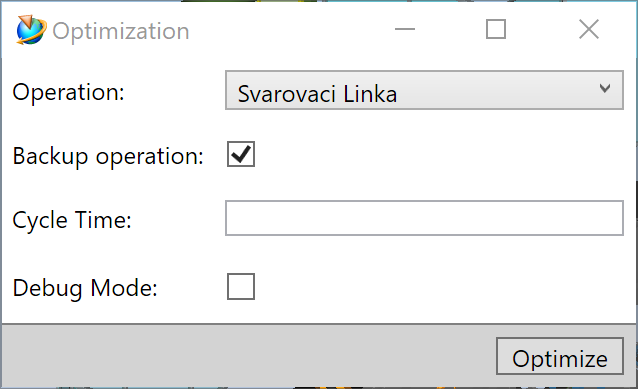
\includegraphics[width=\textwidth]{dialog_beginoptimization}
	\label{fig:DialogBeginOptimization}
\end{figure}

The user first triggers the optimization dialog (see Figure \ref{fig:DialogBeginOptimization}) by clicking on the Optimize button provided by the Plugin. 
The dialog allows the user to adjust parameters of the optimization process. 
First, the system presents him with the operation which should be optimized, which is the operation he had currently set the as the active operation so that he has a chance to adjust this before starting the operation process. In the following text, I will refer to this operation as the root operation.
The user is also presented with the choice to optionally backup the operation which will create a copy of the root operation and then set the duplicate as the new root.
Setting a specific cycle time in seconds will make the MILP model try to match the cycle time instead of minimizing it.
Lastly, the debug option can provide the user with additional information from the MILP solver, explaining the solution, should he have troubles with the proposed schedule. \\

% TODO Class and namespace info
% TODO Explain why the collisions need to be simulated

When started, the optimization process will first aim to gather data about the root operation. It will first simulate the behavior of the root operation while the robots are set to maximum and minimum speeds to obtain the minimum and maximum duration of the individual child activities.\\

Then an optimization graph is built by analyzing the operation tree. This graph is also augmented with the information about the simulation and any initial collisions the process might have encountered. After this initial batch of data is gathered the optimization cycle can start. In this loop, the graph is given to a solver which proposes a solution. The process adjusts the root operation to match the proposed solution, and the result is simulated. If there are no collisions, we have the best viable solution, and the cycle ends. Otherwise, we advance to the next round. To prevent an infinite loop, this can only be repeated a limited amount of times. \\

When the process finishes the system will display a helpful report (see Figure \ref{fig:DialogOptimizationResult}) presenting the most important information about the solution to the user. In the header the cycle time can be found and the body is filled with a graphical representation of the schedule.  

\begin{figure}[ht]
	\caption{Optimization Result Dialog}
	\centering
	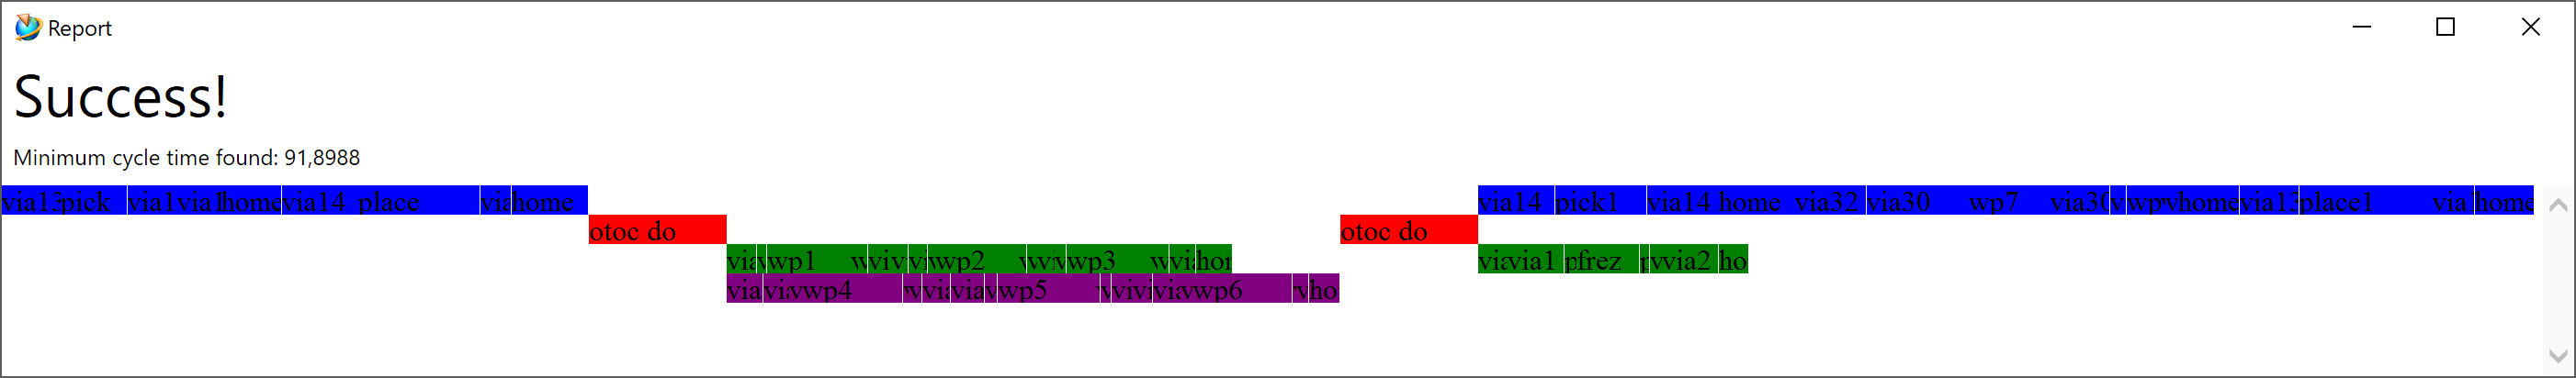
\includegraphics[width=\textwidth]{dialog_optimizationresult}
	\label{fig:DialogOptimizationResult}
\end{figure}

\subsection{Simulation}

The simulation module is a wrapper around the kinematic simulation capability of Process Simulate. It is meant to help with obtaining data about the study which can only be measured. The simulation services are placed in the \emph{Tecnomatix.Optimization.Services.Simulation} and revolve around the \emph{Simulation} class. All new simulations must derive from this class and then can be easily executed. The engine also supports executing multiple simulations simultaneously. \\

To run a simulation, the system needs an operation as an input. Process Simulate will block the UI and compute the movement of the robots in the scope of the given operation, frame by frame. While simulating the player fires events, which the specific simulation can choose to subscribe to if they are relevant for its purpose. Usually, as the playback progresses, the simulation will store some data which when processed will form the output values. Events available range from the simulation being started or ending, operations beginning and ending to the individual time intervals at which the locations of all the objects within the study are computed. \\

A simulation report is a type of simulation, output of which is a data table. This data can be exported into a \emph{csv} file. Reports are useful for debugging or gaining insight into the performance of the activities within the study.

The plugin comes with the following simulations implemented:

\begin{itemize}

\item Collision Simulation. This simulation is checking every frame if there is a collision between the specified collision pairs. The collision pairs can be adjusted in the \emph{Collision Viewer} panel in Process Simulate. The simulation will also track down the responsible operations which controlled the parts that collided.

\item Energy Report. This report captures the simulated energy usage of the robots. Please note that the readings are only as accurate as the robot controller and using a dedicated controller from the manufacturer of the robots is recommended as the readings given by the default robot controller are inaccurate.

\item Joint Speed Report. This report captures the speeds of the joints of the robots while performing the various tasks engulfed in the robotic operation.

\item Duration Simulation. To capture how long it will take for a robot to perform the operation it is first needed for a simulation to run. This information will be captured by Process Simulate afterward, but if any changes happened to the study, it might be inaccurate. For this reason, to obtain accurate readings, this simulation will capture the durations right after the simulation finishes. It is also able to adjust the speed of the robots before running the simulation and restore the original values when done. 

\item Operation Speed Report. This report extracts the speeds the robots are set to run at while executing the particular operations. 

\end{itemize}

\subsection{Graph}

Putting together the optimization graph which serves as the model of the study is one of the most fundamental aspects of the optimization process. It takes a compound operation as an input and traverses all of its descendants transforming it into a flat structure. It also has to analyze the dependencies of the operations and how would it operate in a production cycle. \\

This functionality is being provided by the \emph{GraphVisualizationService} which is located in the \emph{Tecnomatix.Optimization.Services} namespace. It can generate a graph either at bottom-most level of points or one level higher, at the level of paths. For the optimization process used in the point level graph we use the point level graph.\\

First, the optimization graph is filled with vertexes which are the children of the root operation lying at the desired level, grouped by the robot which is assigned to perform them. In each group, the operations are ordered and a so-called "robot loop" is created, by linking the operations together in pairs, each one with the next. One exception to this rule is the edge between the first and the last operation, which are linked by a "robot loop reset" edge instead. \\

\begin{figure}[ht]
	\caption{Projection of the operation tree onto a flat layer}
	\centering
	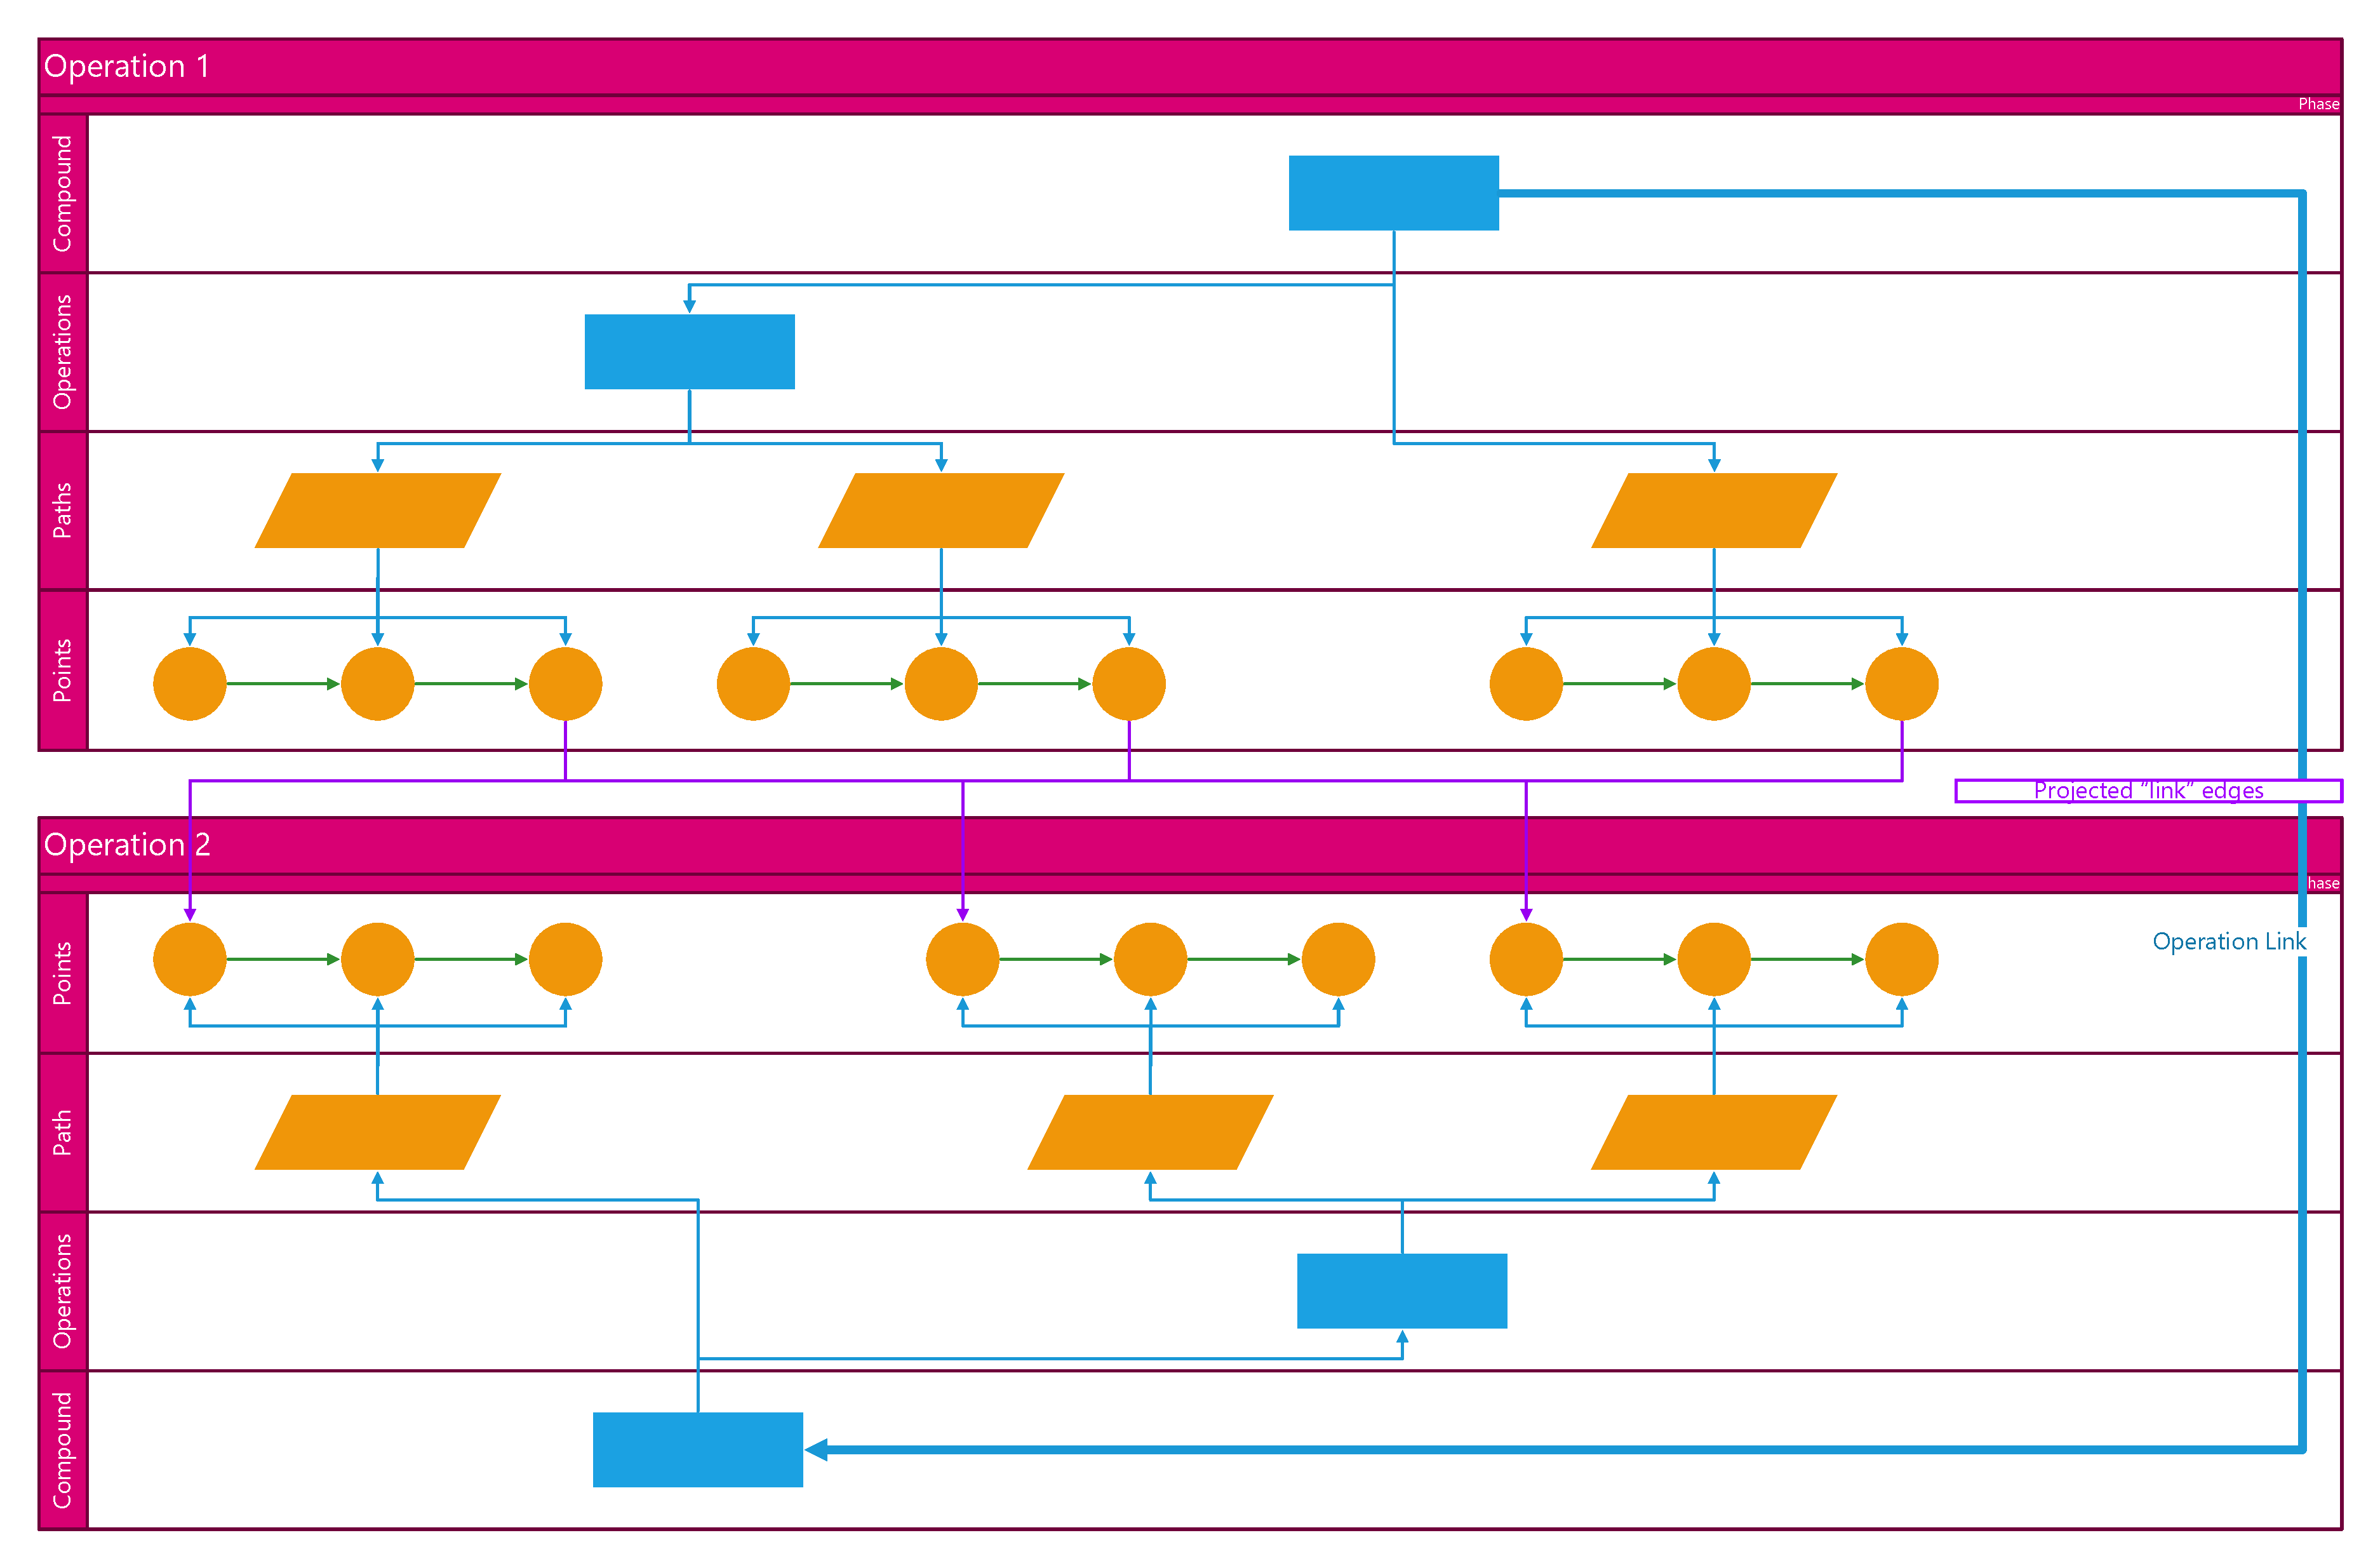
\includegraphics[width=1\textwidth]{graphprojection.pdf}
	\label{fig:GraphProjection}
\end{figure}

The hardest part of the graph creation are the "link" edges which can appear at any level in the operation tree. Since we are flattening the tree into a graph, we need to project them into this new structure. 
This process is different whether we flatten to the level of paths or points.  \\

Let’s say that $descendants(x)$ is a function which returns all descendants on the level of paths (for example on Figure \ref{fig:GraphProjection}, if Operation 1 was given as an input to this function, output of the function would be only the children in the frame "Paths"). Next we need to define the function $first(x)$ which returns the first child (a point) of path $x$ and $last(x)$ returns the last child of $x$.\\

In the first case, it is possible to just find all the descendants at the level of paths of the source of the link $l = (source, target)$ and of the target of the link.
Then we compute the Cartesian product of these two sets $S = descendants(source), T = descendants(target), P = S \times T$. 
For each item in the set $\forall (from, to) \in P$ we create a new link of type "link" which leads from the vertex $source$ to the vertex $target$ in the graph. 
These nodes are guaranteed to exist if the link leads inside the root operation. 
If it leads outside its is ignored because it wouldn't have any impact on the run of the operation. \\

In the latter case, when creating a graph at the level of points, the situation is similar, however, after forming the Cartesian product, we have to select the correct points from the paths. A custom recursive function \emph{ProjectOntoGraph} achieves this. The projection which is a result of the function is illustrated in Figure \ref{fig:GraphProjection}. This function first creates the Cartesian product $P = S \times T$ on the path level, as in the previous case. Then it selects the last or first point $\forall (from, to) \in P: edge = (last(from), first(to))$, depending if the set is coming from a source or a target operation respectively. And then create the corresponding $edge$ in the graph. For example on Figure \ref{fig:GraphProjection} this function would project the blue operation link into the nine purple edges shown in the middle of the diagram.

\subsection{Regulator}

% Intro

The regulator is the main ingredient in the process responsible for taking the output of the optimization and adjusting the operation accordingly. Since how the component works and how its used is very closely tied together, I will explain both in this section. But before we jump to the algorithms we need to realize a few unintuitive facts which we determined experimentally. \\

\begin{figure}[ht]
	\caption{Relation of operation duration to robot speed}
	\centering
	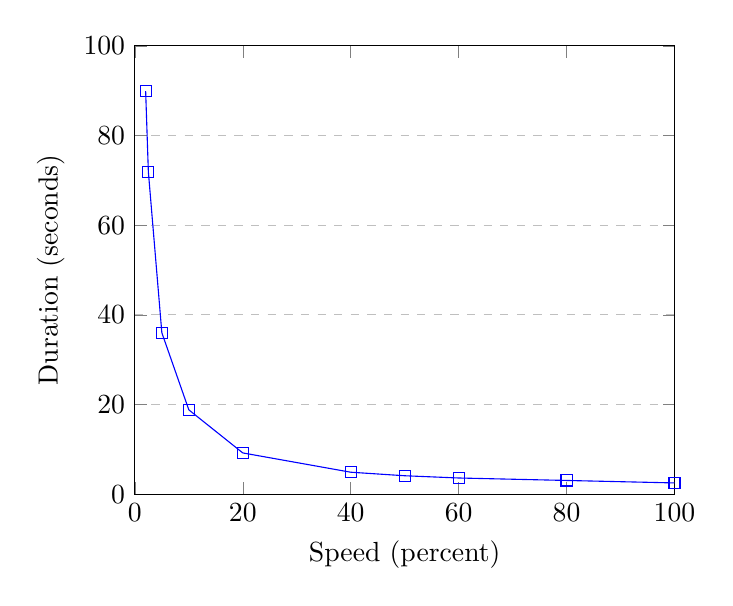
\begin{tikzpicture}
\begin{axis}[
%    title={Relation of operation duration to robot speed},
    xlabel={Speed (percent)},
    ylabel={Duration (seconds)},
    xmin=0, xmax=100,
    ymin=0, ymax=100,
    xtick={0,20,40,60,80,100},
    ytick={0,20,40,60,80,100},
    legend pos=north west,
    ymajorgrids=true,
    grid style=dashed,
]
 
\addplot[
    color=blue,
    mark=square,
    ]
    coordinates {
    (100, 2.5)(80, 3.05)(60, 3.6)(50, 4.1)(40, 4.89)(20, 9.19)(10, 18.8)(5, 36)(2.5, 71.93)(2, 89.9)
    };
\end{axis}
\end{tikzpicture}
	\label{fig:SpeedVsDuration}
\end{figure}

Firstly, as you can see in Figure \ref{fig:SpeedVsDuration}, the relation between duration, which the optimization algorithm calculates, and speed which we need to set for the robots, isn't linear. Unfortunately, the curve also varies from robot to robot and from operation to operation which means the value can't be calculated at all. This challenge we tackle by using a modified interpolation search with a simulation to check what is the actual duration. \\

The second challenge stems from the fact that movement operations can have different precision associated with them. For example, when moving around a corner when the precision requirements are minimal, we can set the operation zone as "coarse" which will allow the robot to move to the next operation after reaching a region around the point specified by a configured tolerance. As opposed to a "fine" zone which will require the robot to move precisely to the specified point and only then it can advance to the next operation. Due to this, the speed of an operation can influence the following operation, and some operations are effectively skipped which implies that adjusting their speed will not change the duration. To address this, I added an upper bound to the MILP model for the operation duration. An operation which is being skipped will then have $\underline{d} = d = \overline{d}$, consequently the optimization engine won't try to adjust this operations duration and therefore its speed. \\

% Class and namespaces
To use the regulator to adjust speeds of an operation we first need to instantiate the \emph{OperationDurationRegulator} class located in the \emph{Tecnomatix.Optimization.Services.Regulation} namespace. First, we need to set the desired processing durations of the points which can be achieved by the \emph{SetBlockDuration} method. Please note that the regulator is designed to adjust multiple operations at the same time because the process needs simulations to check that the adjusted speed resulted in the correct duration. Since simulations are by far the most expensive process, it is a good practice to use the least amount of simulations as possible. The regulator can also adjust operations in blocks in case it didn't make sense to adjust the operation individually, but only the cumulative duration was important. In this case, all the operations in the block will be adjusted to the same speed, and the sum of their durations will be matched to the specified desired duration. After the regulator has all the data, we can begin the calibration process by calling the \emph{Adjust} method on the instance of the regulator class. This is a blocking operation due to the fact that the simulations are blocking the UI thread. \\

% How it works

First of all the regulator holds a lower and upper bound for the speed and duration of each operation. These bounds are set to a speed of 1 (minimum) and the speed of 100 (maximum) and the durations observed for those speeds. Similarly to an interpolation search, the regulator will iterate until it finds an acceptable solution or decides that it is impossible or impractical to continue. In the loop, the first action is to make a prediction of the speed based on the upper and lower bounds and the desired duration. At first, I considered linear interpolation (Equation \ref{eq:LinearInterpolationPrediction}), but because the relation isn't linear as shown on Figure \ref{fig:SpeedVsDuration}, binary halving (Equation \ref{eq:BinaryPrediction}) was used instead because it should converge in fewer iterations in most cases. \\

\begin{equation} \label{eq:LinearInterpolationPrediction}
    prediction = S_{min} + \frac{D}{D_{max}-D_{min}} \times (S_{max}-S_{min})
\end{equation}

\begin{equation} \label{eq:BinaryPrediction}
    prediction = \frac{S_{min} + S_{max}}{2}
\end{equation}

After the prediction is made for all of the blocks which are being adjusted, they're tested by a simulation. Then, based on the simulations results, either the upper or the lower bound of each block is adjusted. \\

% TODO Rephrase the last sentence and point out this is being done in batches
% TODO Why not motion time
% ^ check that

Some readers, aquainted with Process Simulate, might be wondering why we don't convert the movement type of the operation to from joint speed to motion type and write the proposed duration in there. The reason is that the motion type duration only affects the duration of the movement and any OLP commands or welding action take extra time on top of that. Ideally if we could find out the length of the static part we could subtract it and still write the motion type. Alas there is no way to determine the length of the two parts and therefore we can't use that feature and have to ascertain the joint speed by simulation. \\

\subsection{Generator}

% Intro
% Class and namespaces
% How it works
% Implemented features

The generator piece does as the name suggests. It allows for the programatic generation of random optimization graphs which can be used for automated testing. These graphs are not guaranteed to be feasible. \\

Random graphs can be generated using the \emph{GraphGenerationService} located in the \emph{Tecnomatix.Optimization.Services.Generation} namespace. \\

Input to the routine are three parameters which control the size and density of the graph. The parameters are $robots$ which is the number of robot loops in the graph, $operationsPerRobot$ which specifies the number of operations in each loop $\pm variance$. After this trivial graph is created the process will aim to expand the graph to mirror a real life scenario. An $operationsPerRobot$ random dependencies between robots are inserted and the same amount of collisions are artificially created. \\

% TODO virtual tx representations